\ylDisplay{Luup} % Ülesande nimi
{Valter Kiisk} % Autor
{lõppvoor} % Voor
{2016} % Aasta
{G 6} % Ülesande nr.
{7} % Raskustase
{
% Teema: Geomeetriline-optika
\ifStatement
Kui asetada poolkera-kujuline klaaskeha (lääts) tasapinnalise poolega vastu paberit, on võimalik vähemalt läätse keskosa ümbruses näha paberi pinna suurendatud kujutist. Kui mitmekordne kujutis saadakse, vaadeldes kauguselt, mis on hulga suurem läätse mõõtmetest? Klaasi murdumisnäitaja $n=\num{1.5}$.
\pagebreak
\fi


\ifHint
Poolkera kumera pinna keskosa võib vaadelda omaette õhukese läätsena, mille fookuskaugus ja kaugus paberi pinnast määravad kujutise suurenduse. Läätse fookuskauguse leidmiseks on kasulik vaadelda valguskiirt, mis liigub paralleelselt optilise peateljega. Pärast läätses murdumist koondub kiir fookusesse.
\fi


\ifSolution
Poolkera kumera pinna keskosa võib vaadelda omaette õhukese läätsena, mille fookuskaugus $f$ ja kaugus paberi pinnast (võrdne kumerpinna raadiusega $R$) määravad kujutise suurenduse. Selle ekvivalentse läätse fookuskauguse määramiseks vaatleme valguskiirt, mis liigub paralleelselt optilise peateljega ja pärast murdumist koondub fookusesse (vt joonis). Kui valguskiir levib optilise peatelje lähedal, siis kõik murdumisel tekkivad nurgad on väikesed, nii et saame tingimuse
\[
\alpha R\approx f\varphi.
\]
Ilmselt
\[
\varphi = \alpha - \beta=\alpha-\alpha/n=\alpha(1-1/n).
\]
Nende seoste kombineerimisel nurgad taanduvad välja ja saame $f=nR/(n-1)$. Ilmselt eseme (paberi pinna) kaugus läätsest on $R$, kusjuures $f > R$, järelikult tekib näiline kujutis kusagil paberi taga. Kõik kaugused on siiski $R$ suurusjärgus, seega suurelt distantsilt silmaga vaadeldav suurendus (st nurksuurendus) on praktiliselt sama mis joonsuurendus $y/y_0$. Kujutise konstrueerimisel tekkivatest sarnastest kolmnurkadest saame
\[
\frac{y}{y_0}=\frac{f}{f-R}=n=\num{1.5}.
\]

\begin{center}
	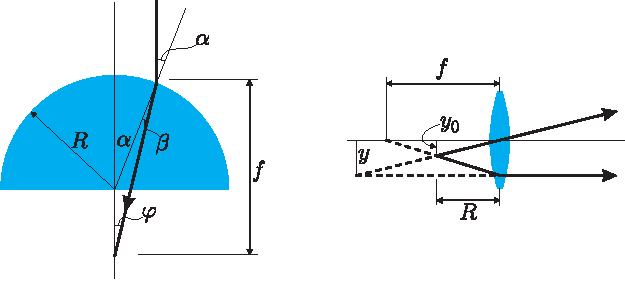
\includegraphics[scale=1.2]{2016-v3g-06-luup-lah}
\end{center}
\fi


\ifEngStatement
% Problem name: Magnifier
If you place the flat side of a hemispherical glass object (lens) against a paper, it is possible to see a magnified image of the paper’s surface around the center of the lens. How many times is the image bigger than the object if you are observing at a distance that is much bigger than the dimensions of the lens? The refractive index of glass is $n=\num{1.5}$.
\fi


\ifEngHint
The middle part of the hemisphere’s round surface can be looked at as a separate thin lens. The focal point and the distance from the paper of this lens would determine the magnification of the image. To find the focal point of the lens it is useful to observe a light ray that moves parallel to the optical axis. After the refracting in the lens the ray focuses in the focal point.
\fi


\ifEngSolution
The central region of the hemisphere’s convex surface can be looked at as a separate thin lens. Its focal length $f$ and distance from the paper’s surface (equal to the radius $R$ of the convex surface) determine the magnification of the image. To determine the focal length of the lens equivalent to the hemisphere we observe a light ray that moves parallel to the optical axis and after refraction converges to the focal point (see figure). If the light ray travels close to the optical axis then all the angles occurring during refraction are small, meaning we get the condition
\[
\alpha R\approx f\varphi.
\]
Probably
\[
\varphi = \alpha - \beta=\alpha-\alpha/n=\alpha(1-1/n).
\]
Combining these relations the angles cancel out and we get $f=nR/(n-1)$. The distance of the object (paper’s surface) is probably $R$, moreover $f > R$, therefore a virtual image appears somewhere behind the paper. All the distances nevertheless have the same order of magnitude as $R$, thus, a magnification looked at at a great distance (meaning angular magnification) is practically the same as a linear magnification $y/y_0$. From the similar triangles that form during the construction of the image we get
\[
\frac{y}{y_0}=\frac{f}{f-R}=n=\num{1.5}.
\]  
\begin{center}
	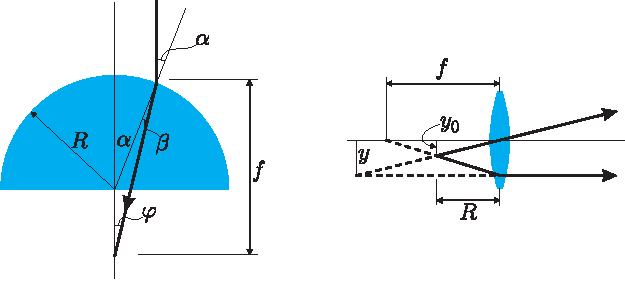
\includegraphics[scale=1.2]{2016-v3g-06-luup-lah}
\end{center}
\fi
}